\scanpage{34}
% archive sheet number: 33
% Left-hand page of the open sheet.
\figure{\begin{tikzpicture}\draw (0,0)--(1.2,0);\draw (0.05,.13)--(1.3,.13);\end{tikzpicture}}
Passant à la limite sur des $S$ de plus en plus {\unsure{grands|petits}} (et {\unsure{faisceautisant}} sur $Y$, pour pouvoir le faire) on trouve un \inserted{pro $Y$-}schéma en {\unsure{grps}} ${\unsure{\mathscr{P}|\Phi}}_{\infty\,X/Y}$, \deleted{{\unsure{fini}}} et un \deleted{{\unsure{pro-morphisme}}}\inserted{{\unsure{pro-application}}} rationnelle {\unsure{transverse}} aux fibres de $X/Y$
\[
{\unsure{\varphi|\phi}}_\infty:X\longrightarrow\mathscr{P}_\infty^1
\]
qui sera solution d'un problème universel relatif aux {\unsure{pro-morphismes}} {\unsure{transverses}} aux fibres de $X/Y$ dans les fibrés principaux sous des $Y$-schémas en groupes \inserted{\uline{commutatifs}} de type fini. On aura alors, si ${\unsure{\mathscr{R}|R}}_{X/Y}\deleted{{\unsure{X}}}$ désigne la \uline{{\unsure{cat. fibrée}}} sur $Y$ définie par $X$
\[
\deleted{{\unsure{\underline{H}^1(\mathscr{R})}}}
\left\{\begin{aligned}
\operatorname{Hom}_{{\unsure{Y}}}({\unsure{\mathscr{R}_{X/Y}^1|\mathscr{R}_{X/Y}}},P^1)&\xleftarrow{\sim}\operatorname{Hom}_{Y\text{-}\mathrm{grp}}(\mathscr{P}_\infty^1,P)\\
\underline{H}^0(\mathscr{R}_{X/Y},G)&\xleftarrow{\sim}\deleted{{\unsure{\operatorname{Ext}^0}}}{\unsure{\underline{\operatorname{Hom}}}}_{Y\text{-}\mathrm{grp}}(\mathscr{P}_\infty,G)\\
\underline{H}^1(\mathscr{R}_{X/Y},G)&\xleftarrow{\sim}\operatorname{Ext}^1_{Y\text{-}\mathrm{grp}}(\mathscr{P}_\infty,G)\\
&\text{et sans doute}\\
\underline{H}^i(\mathscr{R}_{X/Y},G)&\xleftarrow{\sim}\operatorname{Ext}^i_{Y\text{-}\mathrm{grp}}(\mathscr{P}_\infty,G)
\end{aligned}\right.
\]
% margin note slanted, beside the brace of the last displays
\margin{{\unsure{isom de|D'où}} faisceaux sur $S$}

\figure{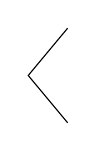
\begin{tikzpicture}\draw (0,1)--(-.5,.4)--(0,-.2);\end{tikzpicture}}
% Right-hand page.
{\unsure{Je voudrais|Je note}} : {\unsure{lier}} les $\operatorname{Ext}^i(\mathscr{P}_{S,X/S},G)$ avec les $\operatorname{Ext}^{{\unsure{i|0}}}(\mathscr{P}^0_{S,X/S},G)$ que l'on considère d'habitude. Le lien se fait par la suite exacte des $\operatorname{Ext}$ {\unsure{déduite}} de
\[
0\longrightarrow\mathscr{P}_S^0\longrightarrow\mathscr{P}_S\longrightarrow\mathbb{Z}\longrightarrow0\tag*{(*)}
\]
donnant donc
\diagram{\begin{tikzcd}[ampersand replacement=\&,column sep=small,row sep=small]
\&\&\operatorname{Hom}(X-S,G)\arrow[d,phantom,"{\tikz[baseline=-.5ex]{\node[rotate=90] {$\simeq$};}}"]\&\&\& H^1(X-S,G)\arrow[d,phantom,"{\tikz[baseline=-.5ex]{\node[rotate=90] {$\simeq$};}}\,?"]\\
0\arrow[r]\&H^0(S,G)\arrow[r]\&\operatorname{Hom}(\mathscr{P}_S,G)\arrow[r]\&\operatorname{Hom}(\mathscr{P}_S^0,G)\arrow[r]\&H^1(S,G)\arrow[r]\&\operatorname{Ext}^1(\mathscr{P}_S,G)
\end{tikzcd}}
\diagram{\begin{tikzcd}[ampersand replacement=\&,column sep=small,row sep=small]
\&\&\&H^2(X-S,G)\arrow[d,phantom,"{\tikz[baseline=-.5ex]{\node[rotate=90] {$\simeq$};}}\,?"]\\
{}\arrow[r]\&\operatorname{Ext}^1(\mathscr{P}_S^0,G)\arrow[r]\&H^2(S,G)\arrow[r]\&\operatorname{Ext}^2(\mathscr{P}_S,G)\arrow[r]\&\cdots
\end{tikzcd}}
\figure{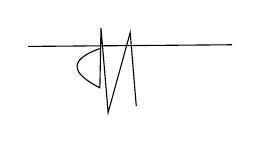
\begin{tikzpicture}[scale=.7]
\draw (0,1.1)--(3.7,1.13);\draw (1.3,1.06)..controls (.7,.85) and (.8,.6)..(1.3,.35)--(1.32,1.43)--(1.45,-.1)--(1.85,1.35)--(1.96,.02);
\end{tikzpicture}}
On notera que dans cette théorie, [du moins pour les {\unsure{courbes}}] on n'a aucun besoin de notion de symbole local, encore moins de la théorie des Jacobiennes locales, qui en un sens semble plus subtile {\unsure{------}}
